% ==============================================================================
% ICEIB 2027 (7th IEEE International Conference on Electronic Communications,
% Internet of Things and Big Data) - Standard IEEE Conference Format
% Conference Website: https://www.iceib.asia/
% Length Specification: 4 to 8 pages (2-column IEEEtran conference format)
% Structure: A-to-Z (A2Z) Academic Writing Style (ref/A2Z_academic_writing_style.md)
% Language: English
% ==============================================================================
\documentclass[conference]{IEEEtran}
\IEEEoverridecommandlockouts

\usepackage{cite}
\usepackage{amsmath,amssymb,amsfonts}
\usepackage{algorithm}
\usepackage{algorithmic}
\usepackage{booktabs}
\usepackage{array}
\usepackage{graphicx}
\usepackage{textcomp}
\usepackage{url}
\usepackage{xcolor}
\usepackage{tikz}
\usetikzlibrary{arrows.meta,positioning,shapes.geometric,fit}

\def\BibTeX{{\rm B\kern-.05em{\sc i\kern-.025em b}\kern-.025em
    T\kern-.1667em\lower.7ex\hbox{E}\kern-.125emX}}

\begin{document}

\title{Food Guardian: A Knowledge-Guided Domain AI Agent for Household Food Inventory Management and Waste Reduction}

\author{
\IEEEauthorblockN{Yi-Fan Chen}
\IEEEauthorblockA{\textit{Department of Computer Science and Engineering}\\
\textit{National Chung Hsing University}\\
Taichung, Taiwan\\
Fannychen0963766865@gmail.com}
}

\maketitle

% ==============================================================================
% ABSTRACT (A-F: Attention Getter, But, Cure, Development, Experiments, Findings)
% ==============================================================================
\begin{abstract}
% [A] Attention Getter
Household food waste drives significant economic loss and environmental strain, largely stemming from forgotten refrigerator or pantry stock, confusion between \emph{Use By} and \emph{Best Before} date labels, and meal planning disconnected from actual home inventory.
% [B] But (Challenge)
Although general-purpose Large Language Model (LLM) chatbots generate fluent recipes, they lack real-time grounding in household stock, cannot enforce transactional stock consistency, and risk fabricating ingredient quantities or unverified safety guidance.
% [C] Cure
To address this gap, we propose \textbf{Food Guardian}, a knowledge-guided domain AI agent that couples LLM tool orchestration with deterministic inventory, portion, and food safety services.
% [D] Development
Built on a four-layer architecture (Streamlit interface, LangGraph-orchestrated Gemini agent with deterministic local fallback, Python domain services, and ACID-compliant SQLite~3 storage), the system constrains language reasoning to seven read-only tools while delegating decimal-exact deduction, calendar-day reminders, three-tier safety triage (\texttt{eligible}, \texttt{review}, \texttt{blocked}), dimension-safe unit conversion, three-mode recipe ranking, and ChromaDB Retrieval-Augmented Generation (RAG) over curated official guidelines to deterministic pipelines.
% [E] Experiments
We evaluate Food Guardian on a controlled 30-case suite (v3.3) spanning inventory, recipe ranking, portion scaling, safety triage, static RAG metadata, and live multi-tool reasoning.
% [F] Findings
All 25 offline deterministic and static checks passed (100\%), and 3 non-RAG live multi-tool cases achieved 100\% valid tool selection accuracy (3/3) with 11.710~s mean successful latency; two RAG-dependent live cases and human quality audits remain pending.
\end{abstract}

\begin{IEEEkeywords}
Domain AI Agent, Household Food Waste, Tool Calling, Retrieval-Augmented Generation (RAG), LangGraph, Inventory Management, Food Safety Triage.
\end{IEEEkeywords}

% ==============================================================================
% I. INTRODUCTION (G-L: General, However, In literature, Judgement, Keypoint, List)
% ==============================================================================
\section{Introduction}

% [G] General
Domestic food management is a persistent sustainability challenge at the household level. According to the United Nations Environment Programme (UNEP) Food Waste Index Report, households represent the largest single contributor to post-harvest food waste globally, discarding hundreds of millions of tonnes of edible food each year~\cite{unep2024}. Every discarded item also forfeits the upstream agricultural water, energy, and cold-chain resources invested across food production and distribution~\cite{fao2019}.

% [H] However
Despite widespread awareness, families routinely discard usable ingredients due to three practical friction points~\cite{tfda_date,foodsafety_4steps}. First, \emph{inventory blindness} arises when items placed in refrigerators, freezers, or pantries are forgotten until spoilage. Second, \emph{date-label misinterpretation} leads consumers to conflate safety-critical \emph{Use By} dates with quality-oriented \emph{Best Before} dates, prompting either premature disposal or unsafe consumption. Third, an \emph{actionability gap} persists when household members know an ingredient is nearing expiration but lack recipes scaled to their exact available quantities and physical units.

% [I] In literature
Prior attempts to mitigate household waste have explored three main directions: manual inventory tracking applications that log expiration dates, computer-vision refrigerator monitors that detect stored items~\cite{schick2023toolformer}, and conversational Large Language Model (LLM) assistants built on tool-calling or Retrieval-Augmented Generation (RAG) frameworks~\cite{yao2023react,lewis2020rag}. Official food-safety portals from the Taiwan Food and Drug Administration (TFDA)~\cite{tfda_freeze,tfda_date} and U.S. FoodSafety.gov~\cite{foodsafety_4steps,foodsafety_charts} also publish structured storage rules, yet these static documents remain disconnected from personal refrigerator state.

% [J] Judgement
Evaluating existing solutions reveals complementary weaknesses. Pure LLM chatbots exhibit strong natural-language fluency but suffer from stock hallucination, arbitrary unit estimation, and an inability to execute atomic database transactions. Conventional manual tracker apps maintain records reliably but lack multi-intent conversational planning and expiry-weighted recipe scaling. Conversely, vision-only prototypes simplify item capture but cannot reliably read occluded package dates or net weights inside opaque containers. Therefore, an effective household assistant must unite real-time ACID inventory tracking with conservative domain rules and constrained AI orchestration.

% [K] Keypoint
To realize this integration, Food Guardian contributes four concrete engineering and algorithmic advances:
\begin{itemize}
    \item \textbf{Transaction-Safe Inventory and Snapshot Logging:} A SQLite~3 persistence layer enforcing \texttt{BEGIN IMMEDIATE} write serialization, fixed-point \texttt{Decimal} arithmetic, immutable completed records, and \texttt{ON DELETE SET NULL} event snapshots so consumption and waste analytics remain consistent.
    \item \textbf{Read-Only LangGraph Tool Calling with Explicit Fallback:} A \texttt{GeminiFoodAgent} state graph binding seven schema-validated read-only tools with auditable execution traces (\texttt{last\_trace}), paired with a deterministic local rule fallback (\texttt{FoodGuardianAgent}) without silent failure masking.
    \item \textbf{Conservative Safety Triage and Dimension-Safe Scaling:} A three-tier pre-filter (\texttt{eligible}, \texttt{review}, \texttt{blocked}) distinguishing \emph{Use By} from \emph{Best Before} labels, coupled with dimension-strict unit normalization and three-mode recipe ranking (\texttt{balanced}, \texttt{ready\_now}, \texttt{expiry\_first}).
    \item \textbf{Source-Attributed RAG and Controlled Evaluation (v3.3):} A local ChromaDB index over 11 verified TFDA and FoodSafety.gov advisories using \texttt{intfloat/multilingual-e5-small}~\cite{wang2024e5}, evaluated across a 30-case benchmark separating API availability from tool-selection accuracy.
\end{itemize}

% [L] List Organization
The remainder of this paper is organized as follows. Section~II categorizes related work across AI tool-calling methods and food-domain knowledge systems, concluding with an Article Summary Table and capability comparison. Section~III presents the Proposed Design, detailing the numbered eight-step architecture, relational schema, agent flowchart, line-numbered pseudocode, mathematical formulations, and a worked execution example. Section~IV reports the Experiment setup, tuning parameters, baseline design, and recorded v3.3 offline and live evaluation results. Finally, Section~V concludes the paper with system scope, deliverables, limitations, and future work, followed by References.

% ==============================================================================
% II. RELATED WORK (M-O: Methods, New Proposed, Organize)
% ==============================================================================
\section{Related Work}

% [M] Methods (1/2 AI Technology + 1/2 Domain Know-how)
\subsection{AI Technology: Tool-Calling Agents and RAG}
Modern domain AI agents overcome static LLM hallucination by combining structured reasoning with external function calls and non-parametric retrieval. ReAct~\cite{yao2023react} interleaved chain-of-thought reasoning with environment actions, demonstrating improved factual grounding over pure prompting. Toolformer~\cite{schick2023toolformer} showed that language models can invoke external APIs and calculators for deterministic computation. To manage multi-turn stateful tool loops, graph-based runtimes such as LangGraph~\cite{langgraph} organize agent and tool nodes as directed cyclic graphs with explicit recursion limits and trace logs. Complementing tool execution, Retrieval-Augmented Generation (RAG)~\cite{lewis2020rag} anchors responses in indexed documents, while multilingual dense embeddings such as Multilingual-E5~\cite{wang2024e5} use asymmetric \texttt{query:} and \texttt{passage:} prefixes to align cross-lingual queries with technical passages.

\subsection{Domain Knowledge: Food Labels, Safety, and Waste Tracking}
On the domain side, domestic food-waste mitigation depends on accurate interpretation of date markings, storage conditions, and portion quantities. Taiwan FDA guidelines~\cite{tfda_date} distinguish packaging \emph{Use By} / expiry dates (safety-critical thresholds under specified storage) from \emph{Best Before} dates (quality indicators), while TFDA freezing advisories~\cite{tfda_freeze} warn that freezing slows rather than indefinitely halts quality degradation and specify safe thawing methods. Similarly, FoodSafety.gov~\cite{foodsafety_4steps,foodsafety_charts} defines refrigerator ($\le 4^\circ\text{C}$) and freezer ($\le -18^\circ\text{C}$) temperature targets, two-hour perishable handling limits, cross-contamination separation, and cold-storage reference windows (e.g., 1--2 days for raw poultry), explicitly noting that appearance and odor alone cannot confirm food safety.

% [N] New Proposed
\subsection{Emerging Hybrid Paradigm: Rule-Constrained Domain Agents}
Recent system designs increasingly shift away from unconstrained generative chatbots toward hybrid architectures in which deterministic domain rules filter candidate actions before an LLM synthesizes explanations. In household food management, delegating unit conversion, expiration arithmetic, and safety exclusion gates to deterministic code ensures that generative creativity never overrides physical inventory facts or safety boundaries.

% [O] Organize (Article Summary Table + SWOT/Capability Matrix + Gap Chain)
\subsection{Comparative Summary and Research Gap}
Tables~\ref{tab:article_summary} and~\ref{tab:swot_matrix} organize representative prior paradigms alongside Food Guardian across problem focus, AI methodology, domain knowledge, datasets, findings, limitations, and SWOT capability trade-offs.

\begin{table*}[t]
\centering
\caption{Article Summary Table Comparing Representative Paradigms and Food Guardian}
\label{tab:article_summary}
\footnotesize
\setlength{\tabcolsep}{3.5pt}
\resizebox{\textwidth}{!}{%
\begin{tabular}{@{}p{1.6cm}p{2.3cm}p{2.3cm}p{2.3cm}p{2.0cm}p{2.5cm}p{2.7cm}@{}}
\toprule
\textbf{Ref. / Paradigm} & \textbf{Problem Addressed} & \textbf{AI Method} & \textbf{Domain Knowledge} & \textbf{Dataset / Source} & \textbf{Key Findings} & \textbf{Limitations} \\
\midrule
Yao et al.~\cite{yao2023react} (2023) & Hallucination in static LLM reasoning & ReAct interleaved thought-action loop & General task-action grounding & QA \& decision benchmarks & Improves factuality via tool observations & Not tailored to ACID inventory or food safety \\
\midrule
Lewis et al.~\cite{lewis2020rag} (2020) & Outdated or unverified parametric knowledge & Dense retrieval + conditioned generation & External document provenance & Knowledge-intensive NLP corpora & Reduces fabrication with source passages & Static retrieval lacks live DB state or unit math \\
\midrule
TFDA \& USDA Guides~\cite{tfda_date,foodsafety_4steps} & Consumer confusion on dates \& cold storage & Rule-based advisory documentation & Use By vs. Best Before, $4^\circ\text{C}$/$-18^\circ\text{C}$ rules & Official regulatory advisories & Clarifies date semantics and handling limits & Passive web text; no inventory or meal linkage \\
\midrule
Manual / Vision Trackers & Forgotten stock \& manual entry effort & Rule filters or object detection & Basic expiration alerts & User logs or food image sets & Tracks stock presence or visual items & Vision misses hidden dates; manual lacks AI planning \\
\midrule
\textbf{Food Guardian (Ours)} & \textbf{Stock-recipe disconnect \& unsafe advice} & \textbf{LangGraph Gemini tool calling + E5 RAG} & \textbf{3-tier safety triage \& unit-safe scaling} & \textbf{SQLite DB + 6 recipes + 11 official docs} & \textbf{25/25 offline checks; 3/3 live tool trace} & \textbf{Manual entry; live RAG \& user trials pending} \\
\bottomrule
\end{tabular}%
}
\end{table*}

\begin{table*}[t]
\centering
\caption{SWOT and Capability Matrix Across Household Food Management Approaches}
\label{tab:swot_matrix}
\footnotesize
\setlength{\tabcolsep}{4pt}
\resizebox{\textwidth}{!}{%
\begin{tabular}{@{}p{2.4cm}p{3.4cm}p{3.4cm}p{3.4cm}p{3.4cm}@{}}
\toprule
\textbf{Approach} & \textbf{Strengths} & \textbf{Weaknesses} & \textbf{Opportunities} & \textbf{Threats / Risks} \\
\midrule
Pure LLM Chatbot & Flexible natural-language cooking dialogue & No live inventory; invents units and stock & Quick recipe brainstorming & Hallucinated safety or missing-item claims \\
\midrule
Manual Inventory App & Reliable CRUD and calendar reminders & No multi-intent AI reasoning or scaling & Simple local record keeping & High user drop-off without meal actionability \\
\midrule
Vision-Only Tracker & Automated camera item detection & Cannot read occluded dates or package mass & Draft item pre-filling & Corrupted stock counts from misclassification \\
\midrule
\textbf{Food Guardian} & \textbf{ACID SQLite, 3-tier triage, 7 read-only tools} & \textbf{Sample recipe set (6 dishes); manual input} & \textbf{Scale to large recipes + OCR draft input} & \textbf{Cloud API 503/429 outages (mitigated by fallback)} \\
\bottomrule
\end{tabular}%
}
\end{table*}

Synthesizing Tables~\ref{tab:article_summary} and~\ref{tab:swot_matrix} yields the core research gap motivating this system:
\begin{equation}
\text{Existing Research} \longrightarrow \text{Limitations} \longrightarrow \text{Research Gap} \longrightarrow \text{Food Guardian}
\end{equation}
Specifically, existing tools either provide conversational flexibility without live database/safety grounding or maintain static records without expiry-aware, unit-safe meal orchestration. Food Guardian bridges this gap by confining LLM reasoning to read-only tool selection over deterministic domain services.

% ==============================================================================
% III. PROPOSED DESIGN (PA-PM)
% ==============================================================================
\section{Proposed Design}

% [PA] Aim, [PB] Based on / Benefit, [PC] Cure / Cause
\subsection{Design Objectives and System Foundations (PA--PC)}
Food Guardian aims (\textbf{PA}) to deliver an end-to-end household food management assistant covering ten functional requirements observed in the system specification (\texttt{DESIGN.md}): validated inventory CRUD (\texttt{FR-01}), active-only edit/delete separation (\texttt{FR-02}), atomic consumption/waste logging (\texttt{FR-03}), calendar-day expiration reminders (\texttt{FR-04}), responsive dashboard UI (\texttt{FR-05}), serving-scaled recipe recommendation (\texttt{FR-06}), attributed food preservation RAG (\texttt{FR-07}), unit-isolated waste analytics (\texttt{FR-08}), conservative safety pre-screening (\texttt{FR-09}), and reproducible offline/live evaluation (\texttt{FR-10}).

The architecture is built upon (\textbf{PB}) a single-host layered stack using Python~3.11+, Streamlit ($\ge 1.66$), SQLite~3, LangGraph ($\ge 1.0$), Google Gemini (\texttt{gemini-2.5-flash}), ChromaDB, and Sentence Transformers. Keeping persistence and domain arithmetic local yields deterministic testability, zero external server overhead, and strict isolation of user inventory files. To cure (\textbf{PC}) the dual failure modes of stock over-deduction and LLM hallucination, \texttt{InventoryService} executes deductions under SQLite \texttt{BEGIN IMMEDIATE} write locks with \texttt{Decimal} arithmetic, while \texttt{GeminiFoodAgent} exposes strictly read-only tools whose numerical outputs cannot be altered by the LLM.

% [PD] Design, [PE] Paper Element, [PG] Graph (Numbered (1)-(8))
\subsection{Numbered Eight-Step Domain AI Agent Architecture (PD, PE, PG)}
Food Guardian organizes execution into four decoupled layers and an eight-step numbered Domain AI Agent pipeline, illustrated in Fig.~\ref{fig:architecture}:
\begin{enumerate}
    \item[\textbf{(1)}] \textbf{User / Application Scenario:} A household member interacts with the Streamlit web UI (\texttt{src/ui/app.py}) to manage stock, review alerts, or ask multi-intent meal and food-safety questions.
    \item[\textbf{(2)}] \textbf{Query / Input Parsing:} \texttt{agent\_chat\_view.py} validates prompt length ($|Q| \le 1200$) and routes the request according to explicit user mode selection (\emph{Gemini + LangGraph} or \emph{Local Rule Fallback}), never silently masking a failed API request as LLM reasoning.
    \item[\textbf{(3)}] \textbf{Planner \& Reasoning Agent:} \texttt{GeminiFoodAgent} (\texttt{gemini\_graph.py}) runs a compiled LangGraph \texttt{StateGraph} (\texttt{START $\rightarrow$ agent $\leftrightarrow$ tools $\rightarrow$ END}) at \texttt{temperature = 0.2}, \texttt{timeout = 35~s}, and \texttt{recursion\_limit = 18}, selecting from seven read-only tools.
    \item[\textbf{(4)}] \textbf{Data Acquisition / Retrieval:} Inventory and safety tools query active SQLite~3 rows via \texttt{InventoryService} and \texttt{ReminderService}, while knowledge queries invoke \texttt{KnowledgeService} or \texttt{FoodRAGService}.
    \item[\textbf{(5)}] \textbf{Analytics \& Portion Engine:} \texttt{portion\_service.py} scales ingredient quantities for $S \in [1, 12]$ servings, performs dimension-safe unit conversion, computes coverage and urgency scores, and ranks dishes under \texttt{balanced}, \texttt{ready\_now}, or \texttt{expiry\_first} mode.
    \item[\textbf{(6)}] \textbf{Domain Knowledge Integration:} \texttt{safety\_service.py} classifies active items into \texttt{eligible}, \texttt{review}, or \texttt{blocked}, and \texttt{FoodRAGService} retrieves top-$k$ passages from ChromaDB (\texttt{food\_guardian\_docs\_v3}) with explicit URLs and verification flags.
    \item[\textbf{(7)}] \textbf{Decision / Recommendation:} The agent synthesizes a Traditional Chinese response strictly preserving tool-computed shortages, unknown-unit warnings, and food-safety disclaimers while recording every call in \texttt{last\_trace}.
    \item[\textbf{(8)}] \textbf{Output \& Interaction:} The chat view renders the grounded answer alongside an expandable tool-call trace; users subsequently record actual consumption or waste through atomic inventory dialogs, feeding \texttt{AnalyticsService}.
\end{enumerate}

Table~\ref{tab:modules} maps each software module (\textbf{PE}) to its responsibility and verification status.

\begin{figure}[t]
\centering
\resizebox{\columnwidth}{!}{%
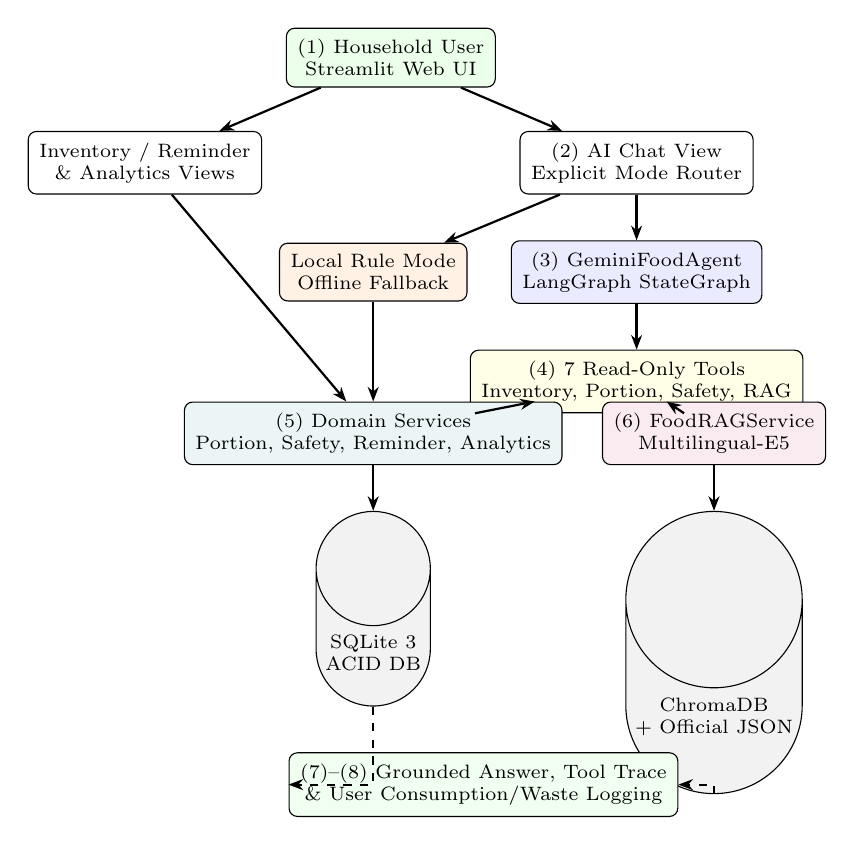
\begin{tikzpicture}[
    node distance=0.52cm and 0.55cm,
    box/.style={draw, rounded corners=3pt, align=center, font=\scriptsize, minimum height=0.62cm, fill=white, inner sep=4pt},
    db/.style={cylinder, shape border rotate=90, draw, minimum height=0.72cm, minimum width=1.15cm, align=center, font=\scriptsize, fill=gray!10},
    arrow/.style={-{Stealth[scale=0.8]}, thick},
    lbl/.style={font=\tiny\bfseries, fill=white, inner sep=1pt}
]
\node[box, fill=green!8] (user) {(1) Household User\\Streamlit Web UI};
\node[box, below left=0.55cm and 0.3cm of user] (invui) {Inventory / Reminder\\\& Analytics Views};
\node[box, below right=0.55cm and 0.3cm of user] (chatui) {(2) AI Chat View\\Explicit Mode Router};

\node[box, below=0.58cm of chatui, fill=blue!8] (agent) {(3) GeminiFoodAgent\\LangGraph StateGraph};
\node[box, left=0.55cm of agent, fill=orange!10] (local) {Local Rule Mode\\Offline Fallback};

\node[box, below=0.58cm of agent, fill=yellow!10] (tools) {(4) 7 Read-Only Tools\\Inventory, Portion, Safety, RAG};

\node[box, below=0.65cm of local, yshift=-0.62cm, fill=teal!8] (services) {(5) Domain Services\\Portion, Safety, Reminder, Analytics};
\node[box, right=0.5cm of services, fill=purple!8] (rag) {(6) FoodRAGService\\Multilingual-E5};

\node[db, below=0.58cm of services] (sqlite) {SQLite 3\\ACID DB};
\node[db, below=0.58cm of rag] (chroma) {ChromaDB\\+ Official JSON};

\node[box, below=0.58cm of sqlite, xshift=1.4cm, fill=green!6] (out) {(7)--(8) Grounded Answer, Tool Trace\\\& User Consumption/Waste Logging};

\draw[arrow] (user) -- (invui);
\draw[arrow] (user) -- (chatui);
\draw[arrow] (invui) -- (services);
\draw[arrow] (chatui) -- (agent);
\draw[arrow] (chatui) -- (local);
\draw[arrow] (agent) -- (tools);
\draw[arrow] (local) -- (services);
\draw[arrow] (tools) -- (services);
\draw[arrow] (tools) -- (rag);
\draw[arrow] (services) -- (sqlite);
\draw[arrow] (rag) -- (chroma);
\draw[arrow, dashed] (sqlite.south) |- (out.west);
\draw[arrow, dashed] (chroma.south) |- (out.east);
\end{tikzpicture}%
}
\caption{Numbered eight-step Domain AI Agent architecture separating semantic tool orchestration (steps 2--3) from deterministic domain computation (steps 4--6) and ACID persistence.}
\label{fig:architecture}
\end{figure}

\begin{table*}[t]
\centering
\caption{Module Responsibility Matrix (Paper Element Mapping)}
\label{tab:modules}
\footnotesize
\setlength{\tabcolsep}{4pt}
\resizebox{\textwidth}{!}{%
\begin{tabular}{@{}llp{5.5cm}l@{}}
\toprule
\textbf{Module / File} & \textbf{Layer} & \textbf{Primary Responsibility} & \textbf{Observed Status} \\
\midrule
\texttt{src/ui/app.py}, \texttt{components/*.py} & Presentation & 5-page dashboard, CRUD/consume/waste dialogs, chat, Plotly analytics & Implemented; team UI review pending \\
\texttt{src/agent/gemini\_graph.py} & Agent & LangGraph \texttt{StateGraph}, 7 read-only tools, trace capture & Live tool trace verified \\
\texttt{src/agent/agent\_core.py} & Agent & Deterministic local rule fallback and legacy OpenAI client path & Unit-tested offline \\
\texttt{src/database/db\_manager.py}, \texttt{schema.sql} & Persistence & SQLite connection lifecycle, \texttt{PRAGMA foreign\_keys = ON}, schema & Implemented & tested \\
\texttt{src/services/inventory\_service.py} & Service & Validated CRUD, \texttt{BEGIN IMMEDIATE} + \texttt{Decimal} consume/waste & Implemented & tested \\
\texttt{src/services/reminder\_service.py} & Service & Calendar-day difference classification (\texttt{1/3/5/7} days) & Implemented & tested \\
\texttt{src/services/portion\_service.py} & Service & Serving scaling, unit conversion, \texttt{classify\_item}, 3-mode ranking & Offline & live trace verified \\
\texttt{src/services/safety\_service.py} & Service & Read-only SQLite safety triage (\texttt{eligible}/\texttt{review}/\texttt{blocked}) & Offline & live trace verified \\
\texttt{src/services/rag\_service.py}, \texttt{build\_rag\_index.py} & Knowledge & Multilingual-E5 embeddings, ChromaDB upsert/query, HTTPS gate & Static & unit tested; live pending \\
\texttt{src/services/analytics\_service.py} & Service & Unit-grouped waste summary, waste reasons, daily trends & Implemented; E-team acceptance pending \\
\bottomrule
\end{tabular}%
}
\end{table*}

% [PF] Formulation
\subsection{Relational Schema and State Formulation (PF)}
The relational model in \texttt{src/database/schema.sql} defines three tables summarized in Table~\ref{tab:schema}. Enumerated fields (\texttt{category}, \texttt{unit}, \texttt{storage\_location}, \texttt{date\_label\_type}, \texttt{status}) are enforced against fixed English constants in \texttt{src/constants.py} while displaying localized Traditional Chinese labels in the UI. Partial consumption or disposal keeps \texttt{status = active}; only when remaining quantity reaches zero does \texttt{status} transition to a read-only \emph{Completed Historical Record} (\texttt{consumed} or \texttt{wasted}), blocking further edits, hard deletes, or deductions. Hard deletion (\texttt{delete\_item}) is permitted only on erroneous \texttt{active} records, while \texttt{consumption\_waste\_logs} preserves denormalized item snapshots with \texttt{ON DELETE SET NULL}.

\begin{table*}[t]
\centering
\caption{SQLite 3 Relational Schema Formulation}
\label{tab:schema}
\footnotesize
\setlength{\tabcolsep}{4pt}
\resizebox{\textwidth}{!}{%
\begin{tabular}{@{}llp{7.8cm}@{}}
\toprule
\textbf{Table} & \textbf{Key Attributes} & \textbf{Integrity Constraints \& Lifecycle Role} \\
\midrule
\texttt{inventory\_items} & \texttt{id}, \texttt{name}, \texttt{category}, \texttt{quantity}, \texttt{unit}, \texttt{purchase\_date}, \texttt{expiry\_date}, \texttt{date\_label\_type}, \texttt{opened\_date}, \texttt{storage\_location}, \texttt{status} & \texttt{CHECK(quantity >= 0)}; \texttt{date\_label\_type} $\in \{\text{use\_by}, \text{best\_before}\}$; \texttt{storage\_location} $\in \{\text{refrigerator}, \text{freezer}, \text{pantry}\}$; \texttt{status} $\in \{\text{active}, \text{consumed}, \text{wasted}\}$. \\
\midrule
\texttt{consumption\_waste\_logs} & \texttt{id}, \texttt{item\_id}, \texttt{item\_name}, \texttt{category}, \texttt{quantity}, \texttt{unit}, \texttt{action\_type}, \texttt{reason}, \texttt{log\_date} & Immutable event snapshot; \texttt{action\_type} $\in \{\text{consumed}, \text{wasted}\}$; \texttt{FOREIGN KEY (item\_id) REFERENCES inventory\_items(id) ON DELETE SET NULL}. \\
\midrule
\texttt{recipe\_recommendations} & \texttt{id}, \texttt{recipe\_title}, \texttt{matched\_ingredients}, \texttt{instructions} & Reserved optional cache table for persisting recommended recipes. \\
\bottomrule
\end{tabular}%
}
\end{table*}

The seven read-only tools bound to \texttt{GeminiFoodAgent} are:
\begin{itemize}
    \item \texttt{query\_active\_inventory\_tool()}: Lists active stock, units, dates, and storage locations.
    \item \texttt{query\_expiring\_items\_tool(days\_ahead)}: Returns items with $0 \le d \le \text{days\_ahead}$ ($0 \le \text{days\_ahead} \le 30$).
    \item \texttt{match\_recipes\_from\_inventory\_tool()}: Ranks top-5 recipes by ingredient overlap and urgency.
    \item \texttt{recommend\_recipes\_for\_servings\_tool(servings, mode)}: Scales recipes ($1 \le \text{servings} \le 12$) under \texttt{balanced}, \texttt{ready\_now}, or \texttt{expiry\_first}.
    \item \texttt{validate\_inventory\_safety\_tool(item\_name)}: Evaluates three-tier safety triage on SQLite stock.
    \item \texttt{get\_food\_preservation\_info\_tool(item\_name)}: Queries JSON sample data (tagged \texttt{verified=False}).
    \item \texttt{search\_food\_knowledge(query, top\_k)}: Queries ChromaDB RAG ($1 \le \text{top\_k} \le 5$).
\end{itemize}

% [PH] How, [PI] Implementation (Flowchart + Line-Numbered Pseudocode)
\subsection{Agent Decision Flowchart and Pseudocode (PH, PI)}
Fig.~\ref{fig:flowchart} shows the runtime decision flowchart handling input validation, explicit mode routing, bounded LangGraph tool loops, error propagation, and trace recording. Algorithm~\ref{alg:agent} formalizes the exact execution loop with line numbers.

\begin{figure}[t]
\centering
\resizebox{\columnwidth}{!}{%
\begin{tikzpicture}[
    node distance=0.45cm and 0.5cm,
    startstop/.style={draw, rounded rectangle, rounded corners=6pt, align=center, font=\scriptsize, fill=green!8, inner sep=4pt},
    process/.style={draw, rectangle, align=center, font=\scriptsize, fill=blue!6, inner sep=4pt},
    decision/.style={draw, diamond, aspect=2.1, align=center, font=\scriptsize, fill=yellow!10, inner sep=2pt},
    arrow/.style={-{Stealth[scale=0.8]}, thick}
]
\node[startstop] (start) {Start: Receive Query $Q$ ($|Q| \le 1200$)};
\node[decision, below=0.42cm of start] (mode) {User Mode =\\Gemini?};
\node[process, left=0.55cm of mode] (local) {Local Rule Mode\\(Keyword Intent +\\Deterministic Tools)};
\node[decision, below=0.48cm of mode] (key) {API Key\\Valid?};
\node[process, right=0.55cm of key, fill=red!8] (err) {Report Explicit Error\\(No Silent Fallback)};
\node[process, below=0.45cm of key] (llm) {Invoke LangGraph \texttt{agent} Node\\($T=0.2$, \texttt{recursion\_limit=18})};
\node[decision, below=0.45cm of llm] (tcall) {Emit\\Tool Calls?};
\node[process, right=0.55cm of tcall] (exec) {Validate Args \& Execute\\Read-Only Tool; Log \texttt{last\_trace}};
\node[startstop, below=0.48cm of tcall] (final) {Return Grounded Response $R$ + Trace $L$};

\draw[arrow] (start) -- (mode);
\draw[arrow] (mode) -- node[above, font=\tiny]{No} (local);
\draw[arrow] (mode) -- node[right, font=\tiny]{Yes} (key);
\draw[arrow] (key) -- node[above, font=\tiny]{No} (err);
\draw[arrow] (key) -- node[right, font=\tiny]{Yes} (llm);
\draw[arrow] (llm) -- (tcall);
\draw[arrow] (tcall) -- node[above, font=\tiny]{Yes} (exec);
\draw[arrow] (exec) |- (llm);
\draw[arrow] (tcall) -- node[right, font=\tiny]{No} (final);
\draw[arrow] (local) |- (final);
\end{tikzpicture}%
}
\caption{Decision flowchart of Food Guardian's agent router, enforcing explicit mode boundaries and auditable tool execution.}
\label{fig:flowchart}
\end{figure}

\begin{algorithm}[t]
\caption{Knowledge-Guided Domain AI Agent Execution}
\label{alg:agent}
\begin{algorithmic}[1]
\REQUIRE User query $Q$, history $H[-8:]$, SQLite state $S_{\text{db}}$, ChromaDB $V_{\text{rag}}$
\ENSURE Grounded response $R$, auditable tool trace $L$
\STATE Validate $Q$ is non-empty and $|Q| \le 1200$; initialize $L \leftarrow []$
\STATE Construct $M \leftarrow [\text{SystemPrompt}] + H[-8:] + [Q]$
\STATE Invoke compiled LangGraph \texttt{StateGraph} ($T=0.2$, limit $18$)
\WHILE{\texttt{AIMessage} contains \texttt{tool\_calls} $C$}
    \FORALL{tool call $c \in C$}
        \STATE Validate bounds ($1 \le \text{servings} \le 12$, $0 \le \text{days} \le 30$, $1 \le k \le 5$)
        \IF{$c$ is \texttt{query\_active\_inventory\_tool} or \texttt{query\_expiring\_items\_tool}}
            \STATE Query active records from $S_{\text{db}}$ and compute $d = \text{expiry\_date} - \text{today}$
        \ELSIF{$c$ is \texttt{validate\_inventory\_safety\_tool}}
            \STATE Apply \texttt{classify\_item} triage (\texttt{eligible}, \texttt{review}, \texttt{blocked})
        \ELSIF{$c$ is \texttt{recommend\_recipes\_for\_servings\_tool}}
            \STATE Scale $q_{\text{req}}$, convert same-dimension units, score via (3)--(5), sort by \texttt{mode}
        \ELSIF{$c$ is \texttt{search\_food\_knowledge}}
            \STATE Encode \texttt{"query: " + q} via Multilingual-E5; retrieve top-$k$ from $V_{\text{rag}}$
        \ENDIF
        \STATE Append $\{\text{tool}, \text{arguments}, \text{result}\}$ to trace $L$
    \ENDFOR
    \STATE Feed \texttt{ToolMessage} payloads back to \texttt{agent} node
\ENDWHILE
\STATE Extract terminal \texttt{AIMessage} text as grounded response $R$
\RETURN $(R, L)$
\end{algorithmic}
\end{algorithm}

% [PM] Math Proof, [PK] Keypoint Contribution
\subsection{Mathematical Formulation and Safety Algorithms (PK, PM)}
Food Guardian enforces exact mathematical definitions across reminder classification, safety triage, portion scaling, recommendation scoring, and waste analytics:

\textbf{1) Calendar-Day Reminder Classification:} Given today's date and threshold $t \in \{1, 3, 5, 7\}$ (default $t = 3$), let $d = \text{expiry\_date} - \text{today}$. \texttt{ReminderService} maps each active item to:
\begin{equation}
\text{Status}(d, t) =
\begin{cases}
\texttt{no\_date}, & \text{if } \text{expiry\_date} = \text{NULL} \\
\texttt{passed\_date}, & \text{if } d < 0 \\
\texttt{expiring\_soon}, & \text{if } 0 \le d \le t \\
\texttt{normal}, & \text{if } d > t
\end{cases}
\end{equation}
An item's \texttt{opened\_date} is tracked independently without fabricating a secondary expiration date.

\textbf{2) Three-Tier Conservative Safety Triage:} In \texttt{classify\_item}, active stock is partitioned conservatively:
\begin{itemize}
    \item \texttt{blocked}: Non-active items, invalid quantities, \texttt{known\_spoiled = True}, malformed ISO dates, or expired \texttt{use\_by} items ($d < 0 \land \text{label} = \texttt{use\_by}$).
    \item \texttt{review}: Items past \texttt{best\_before} ($d < 0 \land \text{label} \neq \texttt{use\_by}$) or lacking a recognized label type; requires human inspection.
    \item \texttt{eligible}: Active items not past their labeled date (or undated items with caution). Crucially, \texttt{eligible} denotes only that no exclusion rule fired, never an edible safety guarantee.
\end{itemize}

\textbf{3) Dimension-Safe Scaling and Three-Mode Ranking:} For target servings $S \in \{1,\dots,12\}$ and recipe base servings $S_{\text{base}} \ge 1$, ingredient demand scales as $q_{\text{req}}(i) = q_{\text{base}}(i) \cdot (S / S_{\text{base}})$. Unit conversion is restricted strictly within identical physical dimensions: mass (\texttt{g} $\leftrightarrow$ \texttt{kg}, factor $1000$), volume (\texttt{ml} $\leftrightarrow$ \texttt{l}, factor $1000$), and count (\texttt{piece}, factor $1$). Non-convertible units (e.g., \texttt{other}) yield status \texttt{unknown} and \texttt{needs\_manual\_quantity\_check = True}; otherwise status is \texttt{enough} ($q_{\text{avail}} \ge q_{\text{req}}$), \texttt{insufficient} ($0 < q_{\text{avail}} < q_{\text{req}}$), or \texttt{missing} ($q_{\text{avail}} = 0$).

For each candidate recipe $r$ matching at least one eligible stock item, normalized coverage and urgency are computed as:
\begin{equation}
\text{coverage}(r) = \frac{|\{i \in r : \text{status}(i) = \texttt{enough}\}|}{|r|}
\end{equation}
\begin{equation}
\text{urgency}(r) = \max_{\substack{i \in r,\, q_{\text{avail}}(i) > 0 \\ e \in \text{eligible}(i),\, 0 \le d_e \le 3}} \left(\frac{3 - d_e}{4}\right)
\end{equation}
with $\text{urgency}(r) = 0$ if no matched stock expires within 3 days. The composite ranking score is:
\begin{equation}
\text{score}(r) = 0.65 \cdot \text{coverage}(r) + 0.35 \cdot \text{urgency}(r)
\end{equation}
Sorting is parameterized by mode: \texttt{balanced} sorts by $(-\text{score}(r), \text{id})$; \texttt{ready\_now} sorts by $(\neg \text{all\_quantities\_sufficient}, -\text{score}(r), \text{id})$; and \texttt{expiry\_first} sorts by $(-\text{urgency}(r), -\text{coverage}(r), \text{id})$ while setting \texttt{can\_make\_now = False} whenever any ingredient is missing, insufficient, or \texttt{unknown}.

\textbf{4) Source-Attributed RAG and Unit-Isolated Waste Rate:} \texttt{FoodRAGService} segments documents exceeding 1,800 characters into 1,200-character chunks, encodes \texttt{"passage: "} prefixes with \texttt{intfloat/multilingual-e5-small}, and enforces via \texttt{build\_rag\_index.py} that all indexed \texttt{official\_*.json} entries carry \texttt{verified == True} and an \texttt{https://} URL. Finally, \texttt{AnalyticsService} aggregates \texttt{consumption\_waste\_logs} strictly within each compatible unit $u$:
\begin{equation}
\text{Waste Rate}_u = \frac{W_u}{C_u + W_u} \times 100\%, \quad \text{for } C_u + W_u > 0
\end{equation}
preventing invalid cross-unit summation across \texttt{g}, \texttt{piece}, and \texttt{l}.

% [PJ] Jump to Example, [PL] Later Simulation
\subsection{Worked Execution Walkthrough (PJ, PL)}
Consider a household inventory on reference date \texttt{2026-11-11} containing Tomatoes (2~pieces, +1~day), Eggs (3~pieces, +5~days), Spinach (1~\texttt{other}, +2~days), Chicken Breast (300~g, +3~days), Milk (1~L, +4~days), and Cabbage (1~piece, +6~days). When a user requests a 2-serving dinner prioritizing expiring items, \texttt{recommend\_recipes\_for\_servings\_tool(servings=2, mode="expiry\_first")} computes:
\begin{itemize}
    \item \emph{Tomato Scrambled Eggs} (base 2 servings: 2 tomatoes, 4 eggs): Tomato $q_{\text{req}} = 2 \le 2$ (\texttt{enough}, $d=1 \Rightarrow \text{urgency} = (3-1)/4 = 0.5$); Egg $q_{\text{req}} = 4 > 3$ (\texttt{insufficient}, missing 1); $\text{coverage} = 0.5$, $\text{score} = 0.65(0.5)+0.35(0.5) = 0.500$. Under \texttt{expiry\_first}, it ranks first to rescue expiring tomatoes, yet \texttt{can\_make\_now = False} explicitly warns that 1 egg is missing.
    \item \emph{Cabbage Scrambled Eggs} (base 2 servings: 0.5 cabbage, 3 eggs): Both ingredients satisfy $q_{\text{avail}} \ge q_{\text{req}}$ ($\text{coverage} = 1.0$, $\text{urgency} = 0$, $\text{score} = 0.650$). Under \texttt{ready\_now}, it ranks first with \texttt{can\_make\_now = True}.
    \item \emph{Chicken Breast Safety Query}: Invoking \texttt{validate\_inventory\_safety\_tool("Chicken Breast")} reads the SQLite record (300~g, \texttt{use\_by} +3~days) and returns \texttt{eligible} alongside a mandatory caution that dates alone cannot certify safety.
\end{itemize}

% ==============================================================================
% IV. EXPERIMENT (Q-V: Quality/Quantity, Related Compare, Setup, Tuning, Results, Verify)
% ==============================================================================
\section{Experiment}

% [Q] Quality & Quantity Metrics, [R] Related Compare Baselines
\subsection{Evaluation Metrics and Baseline Design (Q, R)}
Following the v3.3 evaluation harness (\texttt{evaluation/metrics.py}), system performance is measured using strictly separated deterministic and live metrics:
\begin{itemize}
    \item \textbf{Deterministic Check Pass Rate:} Exact agreement on inventory queries, mode-specific recipe ranking, scaled quantity status/shortage, safety triage states, and static official RAG document metadata.
    \item \textbf{API Success Rate:} Fraction of live LLM queries completing without unrecovered network/API errors ($\text{valid} / N_{\text{attempted}}$).
    \item \textbf{Valid Tool Selection Accuracy:} Fraction of API-successful responses whose \texttt{last\_trace} includes all expected tools ($\text{tool\_passes} / \text{valid}$), kept separate from cloud API availability so transient HTTP 503/429 outages are reported as \texttt{API\_ERROR} rather than model reasoning failures.
    \item \textbf{End-to-End Tool Success Rate & Latency:} $\text{tool\_passes} / N_{\text{attempted}}$, retry counts, and mean successful wall-clock latency (s).
\end{itemize}

Conceptually, Food Guardian is contrasted against two baselines: \textbf{Baseline 1 (Unranked / Static Lookup)} without expiry urgency or mode separation, and \textbf{Baseline 2 (Pure LLM Chatbot)} lacking live SQLite tools, deterministic scaling, and safety triage gates. In contrast, our proposed method combines \texttt{balanced}/\texttt{ready\_now}/\texttt{expiry\_first} deterministic services with LangGraph tool orchestration.

% [S] Simulation Setup, [T] Tuning Parameters
\subsection{Simulation Setup and Tuning Parameters (S, T)}
All evaluation artifacts reside in \texttt{evaluation/cases.json} and \texttt{evaluation/run\_evaluation.py} (v3.3), comprising 30 test cases across six categories (5 cases each): \texttt{inventory} (\texttt{INV-01}--\texttt{INV-05}), \texttt{recipe} (\texttt{REC-01}--\texttt{REC-05}), \texttt{quantity} (\texttt{QUA-01}--\texttt{QUA-05}), \texttt{safety} (\texttt{SAF-01}--\texttt{SAF-05}), \texttt{rag} (\texttt{RAG-01}--\texttt{RAG-05}), and \texttt{multi\_tool} (\texttt{MUL-01}--\texttt{MUL-05}). Offline checks pin \texttt{TODAY = 2026-11-11} against the six-item synthetic fixture and the six demonstration recipes in \texttt{recipes.sample.json}, isolating evaluation from any user SQLite database.

Key system and evaluation parameters (\textbf{T}) are fixed as follows: Gemini model \texttt{gemini-2.5-flash}, \texttt{temperature = 0.2}, model timeout \texttt{35~s}, LangGraph \texttt{recursion\_limit = 18}, bounded transient retry \texttt{max\_retries = 1} with exponential backoff base \texttt{2.0~s} plus $[0, 1]$~s random jitter for HTTP $\{429, 503, 504\}$, default reminder window $t = 3$ days (UI options $\{1, 3, 5, 7\}$), composite score weights $0.65 / 0.35$, and RAG chunk length $1,200$ characters (threshold $> 1,800$).

% [U] Useful Results, [V] Verify
\subsection{Experimental Results and Validity Analysis (U, V)}
Table~\ref{tab:offline} reports the recorded offline results from \texttt{evaluation/results/summary.json} and \texttt{offline\_results.csv}. All 25 offline-evaluable checks passed (100\%), verifying exact unit conversion (\texttt{QUA-03}: 1~L milk $\rightarrow$ 1000~mL available $\ge$ 500~mL required), unconvertible-unit blocking (\texttt{QUA-04}: spinach \texttt{other} $\rightarrow$ \texttt{unknown}), \texttt{use\_by} blocking vs. \texttt{best\_before} review (\texttt{SAF-02}, \texttt{SAF-03}), and static HTTPS source metadata across the 11 documents in \texttt{official\_food\_safety.json} (\texttt{RAG-01}--\texttt{RAG-05}). The five \texttt{multi\_tool} cases were appropriately marked \texttt{NOT\_RUN} offline.

\begin{table*}[t]
\centering
\caption{Recorded Offline Evaluation v3.3 Results (Pinned Date: 2026-11-11)}
\label{tab:offline}
\footnotesize
\resizebox{\textwidth}{!}{%
\begin{tabular}{@{}lcccp{6.2cm}@{}}
\toprule
\textbf{Category} & \textbf{Cases} & \textbf{PASS} & \textbf{NOT\_RUN} & \textbf{Verified Deterministic / Static Scope} \\
\midrule
Inventory (\texttt{INV-01}--\texttt{05}) & 5 & 5 & 0 & Fixture count (6), item lookup, 3-day expiry list, absent-item check \\
Recipe (\texttt{REC-01}--\texttt{05}) & 5 & 5 & 0 & \texttt{ready\_now} vs. \texttt{expiry\_first} vs. \texttt{balanced} ordering \\
Quantity (\texttt{QUA-01}--\texttt{05}) & 5 & 5 & 0 & Egg shortage (\texttt{-1}), \texttt{l}$\rightarrow$\texttt{ml} conversion, \texttt{other} unit guard, missing item \\
Safety (\texttt{SAF-01}--\texttt{05}) & 5 & 5 & 0 & \texttt{eligible}, \texttt{review} (\texttt{best\_before}), \texttt{blocked} (\texttt{use\_by} / spoiled) \\
RAG Static (\texttt{RAG-01}--\texttt{05}) & 5 & 5 & 0 & HTTPS URL \& keyword readiness across 11 official JSON documents \\
Multi-Tool (\texttt{MUL-01}--\texttt{05}) & 5 & 0 & 5 & Requires live LLM tool calling; not executed offline \\
\midrule
\textbf{Total} & \textbf{30} & \textbf{25} & \textbf{5} & \textbf{25/25 Offline Checks Passed (100\%)} \\
\bottomrule
\end{tabular}%
}
\end{table*}

Table~\ref{tab:live} summarizes the recorded live multi-tool run from \texttt{evaluation/results/live\_results.csv}. In accordance with \texttt{select\_live\_cases}, the two RAG-dependent cases (\texttt{MUL-02}, \texttt{MUL-04}) were placed in \texttt{skipped\_cases} because live ChromaDB retrieval requires an independently verified RAG index evaluation. Across the three non-RAG multi-tool prompts (\texttt{MUL-01}, \texttt{MUL-03}, \texttt{MUL-05}), the Gemini + LangGraph agent achieved 3/3 API success (100\%) and 3/3 valid tool selection accuracy (100\%), triggering one transient retry on \texttt{MUL-01} with a mean successful response latency of 11.710~s.

\begin{table*}[t]
\centering
\caption{Recorded Live Gemini Multi-Tool Evaluation Results (v3.3)}
\label{tab:live}
\footnotesize
\setlength{\tabcolsep}{4pt}
\resizebox{\textwidth}{!}{%
\begin{tabular}{@{}lccccll@{}}
\toprule
\textbf{Case ID} & \textbf{Status} & \textbf{Retries} & \textbf{Latency (s)} & \textbf{Tool Pass} & \textbf{Invoked Tools (\texttt{last\_trace})} & \textbf{Human Audit Field} \\
\midrule
\texttt{MUL-01} & PASS & 1 & 26.693 & True & \texttt{query\_expiring\_items\_tool}, \texttt{recommend\_recipes\_for\_servings\_tool} & \texttt{REQUIRES\_HUMAN\_REVIEW} \\
\texttt{MUL-03} & PASS & 0 & 3.668 & True & \texttt{query\_active\_inventory\_tool}, \texttt{recommend\_recipes\_for\_servings\_tool} & \texttt{REQUIRES\_HUMAN\_REVIEW} \\
\texttt{MUL-05} & PASS & 0 & 4.769 & True & \texttt{recommend\_recipes\_for\_servings\_tool}, \texttt{validate\_inventory\_safety\_tool} & \texttt{REQUIRES\_HUMAN\_REVIEW} \\
\midrule
\textbf{Summary} & \textbf{3/3} & \textbf{1} & \textbf{11.710} & \textbf{100\%} & \textbf{API Success: 100\%; Tool Acc: 100\%} & \textbf{MUL-02, MUL-04 skipped (RAG)} \\
\bottomrule
\end{tabular}%
}
\end{table*}

For rigorous scientific validity (\textbf{V}), we emphasize three boundaries: (1) tool-trace passes prove that the LLM selected the required tools, whereas \texttt{task\_completion\_review} and \texttt{groundedness\_review} remain explicitly marked \texttt{REQUIRES\_HUMAN\_REVIEW}; (2) \texttt{RAG-01}--\texttt{RAG-05} offline checks verify source metadata readiness rather than semantic retrieval precision; and (3) separate early-stage UI test counts documented during team development are not combined with the v3.3 suite metrics.

% ==============================================================================
% V. CONCLUSION (W-Z: What Proposed, eXcel, Yields, Zen)
% ==============================================================================
\section{Conclusion}

% [W] What Proposed
This paper presented \textbf{Food Guardian}, a knowledge-guided domain AI agent designed to reduce household food waste by uniting inventory tracking, date-label awareness, explainable recipe recommendation, and consumption/waste analytics. By decoupling LangGraph-based Gemini tool selection from deterministic Python domain services and ACID-protected SQLite~3 transactions, Food Guardian prevents unsupported stock fabrication, unsafe unit coercion, and concurrent over-deduction while enforcing conservative three-tier food safety triage.

% [X] eXcel (Scope & Strengths)
Scoped deliberately as a single-household local prototype, the system excels at auditable, rule-constrained decision support: every shortage count, unit conversion, date boundary, and safety status is computed deterministically and exposed alongside an inspectable \texttt{last\_trace}, complemented by an explicit offline local rule fallback.

% [Y] Yields (Deliverables)
The project delivers a reproducible open-source implementation comprising the Streamlit application (\texttt{src/ui/}), SQLite schema and service modules (\texttt{src/database/}, \texttt{src/services/}), LangGraph and fallback agent modules (\texttt{src/agent/}), nine automated pytest suites (\texttt{tests/}), the 30-case v3.3 evaluation harness with recorded CSV/JSON outputs (\texttt{evaluation/}), and environment/index setup scripts (\texttt{.env.example}, \texttt{requirements.txt}, \texttt{scripts/build\_rag\_index.py}).

% [Z] Zen (Limitations & Future Work)
Future work will address four remaining frontiers: (1) expanding \texttt{recipes.sample.json} (currently 6 demonstration dishes) to larger curated recipe corpora with multi-dish shared-inventory optimization; (2) completing live RAG evaluation on \texttt{MUL-02} and \texttt{MUL-04} together with structured human grading of answer groundedness and safety phrasing; (3) integrating optional receipt OCR or camera-assisted detection as human-confirmed draft inputs to reduce manual entry friction for ambiguous \texttt{other}/\texttt{pack} units; and (4) conducting longitudinal household trials using \texttt{AnalyticsService} to empirically measure long-term waste reduction.

% ==============================================================================
% REFERENCES
% ==============================================================================
\begin{thebibliography}{00}
\bibitem{unep2024} United Nations Environment Programme, ``Food Waste Index Report 2024,'' Nairobi, Kenya, 2024. [Online]. Available: \url{https://www.unep.org/resources/publication/food-waste-index-report-2024}
\bibitem{fao2019} Food and Agriculture Organization of the United Nations (FAO), ``The State of Food and Agriculture 2019: Moving Forward on Food Loss and Waste Reduction,'' Rome, Italy, 2019.
\bibitem{yao2023react} S. Yao, J. Zhao, D. Yu, N. Du, I. Shafran, K. Narasimhan, and Y. Cao, ``ReAct: Synergizing reasoning and acting in language models,'' in \emph{Proc. Int. Conf. Learn. Represent. (ICLR)}, 2023.
\bibitem{schick2023toolformer} T. Schick, J. Dwivedi-Yu, R. Dess\`{i}, R. Raileanu, M. Lomeli, E. Hambro, L. Zettlemoyer, N. Cancedda, and T. Scialom, ``Toolformer: Language models can teach themselves to use tools,'' in \emph{Adv. Neural Inf. Process. Syst. (NeurIPS)}, vol. 36, 2023.
\bibitem{lewis2020rag} P. Lewis et al., ``Retrieval-augmented generation for knowledge-intensive NLP tasks,'' in \emph{Adv. Neural Inf. Process. Syst. (NeurIPS)}, vol. 33, pp. 9459--9474, 2020.
\bibitem{wang2024e5} L. Wang, N. Yang, X. Huang, L. Yang, R. Majumder, and F. Wei, ``Multilingual E5 text embeddings: A technical report,'' \emph{arXiv preprint arXiv:2402.05672}, 2024.
\bibitem{langgraph} LangChain AI, ``LangGraph: Build resilient language agents as graphs,'' 2024. [Online]. Available: \url{https://www.langchain.com/langgraph}
\bibitem{tfda_freeze} Taiwan Food and Drug Administration (TFDA), ``Frozen food storage and safe thawing guidelines,'' Ministry of Health and Welfare, Taiwan. [Online]. Available: \url{https://www.fda.gov.tw/TC/siteListContent.aspx?id=51248&sid=13694}
\bibitem{tfda_date} Taiwan Food and Drug Administration (TFDA), ``Guidelines for evaluating expiration dates of packaged foods (Use By vs. Best Before),'' Ministry of Health and Welfare, Taiwan. [Online]. Available: \url{https://foodlabel.fda.gov.tw/FdaFrontEndApp/OtherData/Edit?ClType=2&SystemId=39148789-b32f-4e57-8406-6e7d9145f013}
\bibitem{foodsafety_4steps} U.S. Department of Health and Human Services, ``4 Steps to Food Safety,'' FoodSafety.gov. [Online]. Available: \url{https://www.foodsafety.gov/keep-food-safe/4-steps-to-food-safety}
\bibitem{foodsafety_charts} U.S. Department of Health and Human Services, ``Cold Food Storage Chart,'' FoodSafety.gov. [Online]. Available: \url{https://www.foodsafety.gov/food-safety-charts/cold-food-storage-charts}
\end{thebibliography}

\end{document}
